\documentclass[11pt, oneside]{article}
\usepackage[letterpaper, margin=2cm]{geometry}
\usepackage{MATH667}

\begin{document}
\noindent \textbf{\Large{Caleb Logemann \\
MATH667 Hyperbolic Partial Differential Equations \\
Homework 3
}}

%\lstinputlisting[language=MATLAB]{H01_23.m}
Solve Burgers' equation
\begin{gather}
    u_t + \p{\frac{u^2}{2}}_x = 0 \qquad x \in \br{-5, 5} \\
    u(x, 0) = 
    \begin{cases}
      u_l & x \le 0 \\
      u_r & x > 0
    \end{cases}
\end{gather}
with the following Riemann initial data sets.

\begin{enumerate}
  \item[(a)]
    \[
      u(x, 0) =
      \begin{cases}
        1 & x \le 0 \\
        -0.5 & x > 0
      \end{cases}
    \]

  \item[(b)]
    \[
      u(x, 0) =
      \begin{cases}
        -1 & x \le 0 \\
        0.5 & x > 0
      \end{cases}
    \]
\end{enumerate}
\begin{enumerate}
  \item % #1 Done
    Determine the exact solutions for all $t > 0$.
    \begin{enumerate}
      \item[(a)]
        In this case $u_l > u_r$, so the solution is a shock that propogates
        with speed
        \[
          s = \frac{f(u_l) - f(u_r)}{u_l - u_r} = \frac{1}{2} \p{u_l + u_r} = \frac{1}{2} \p{1 - 0.5} = 0.25
        \]
        Therefore the exact solution is
        \[
          u(x, t) =
          \begin{cases}
            1 & x \le 0.25 t \\
            -0.5 & x > 0.25 t
          \end{cases}
        \]

      \item[(b)]
        In this case $u_l < u_r$ so the solution is a rarefaction.
        Therefore the left side will move with speed $u_l$, the right side
        will move with speed $u_r$, and the middle with connect the sides linearly.
        \[
          u(x, t) =
          \begin{cases}
            -1 & x \le -t \\
            x/t & -t < x < 0.5t \\
            0.5 & 0.5 t \le x
          \end{cases}
        \]
    \end{enumerate}

  \item % #2 Done
    The following function implement the Roe scheme, the Lax-Friedrichs scheme,
    and both the standard and Richtmyer versions of the Lax-Wendroff method.
    I implemented both the standard Lax-Wendroff and the Richtmyer methods
    because the Lax-Wendroff method was giving me the wrong weak solution, while
    the Richtmyer was giving me the entropy solution in the rarefaction case.
    \lstinputlisting[language=MATLAB]{roe.m}
    \lstinputlisting[language=MATLAB]{laxFriedrichs.m}
    \lstinputlisting[language=MATLAB]{laxWendroff.m}
    \lstinputlisting[language=MATLAB]{richtmyer.m}

    The following script uses these functions to solve the Burgers equation for
    the shock and rarefaction case.
    The following images are produced.
    All of these images are zoomed in to the area of interest.
    Note that in rarefaction case the Richtmyer Lax-Wendroff method produces
    just a rarefaction were the standard Lax-Wendroff produces a shock and
    rarefaction.
    Also the oscillations in the Lax-Wendroff method cause this shock to be out
    of proportion.
    \begin{center}
      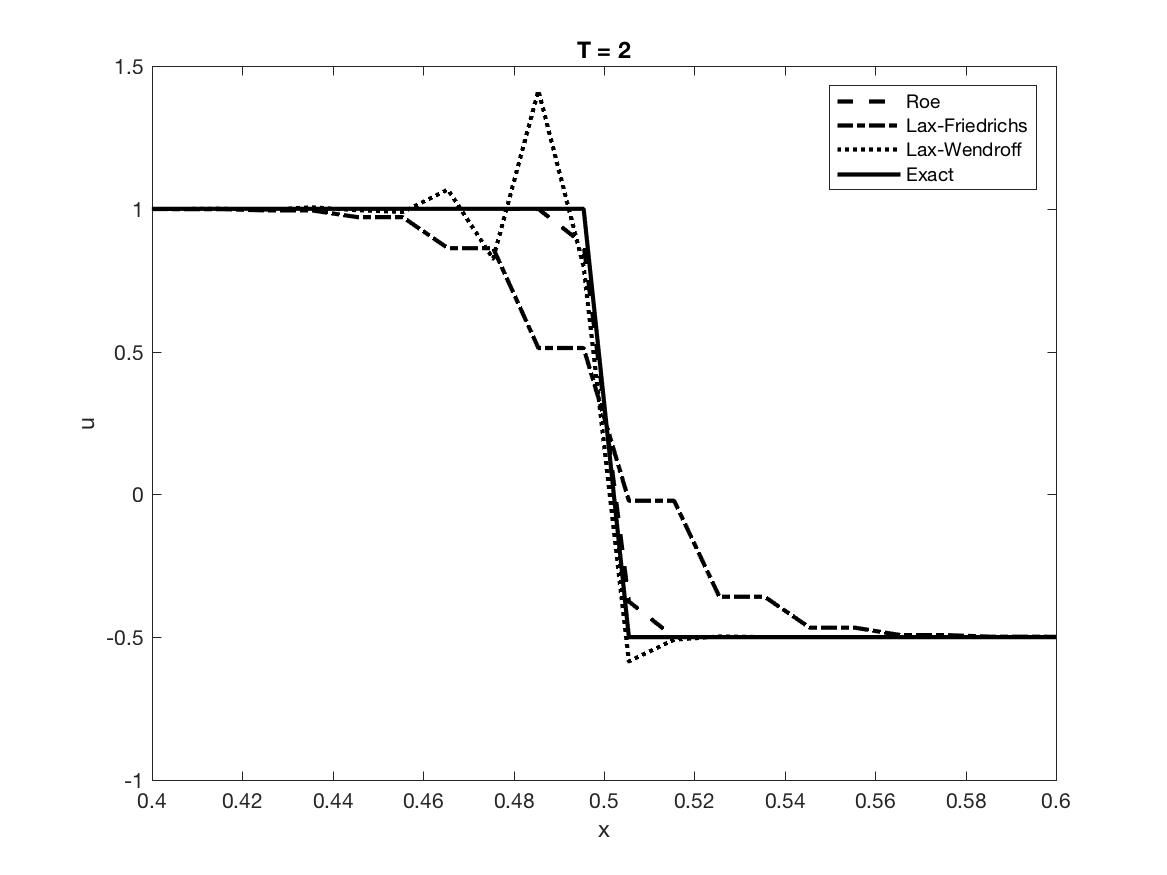
\includegraphics[scale=0.5]{Figures/03_01.png}
      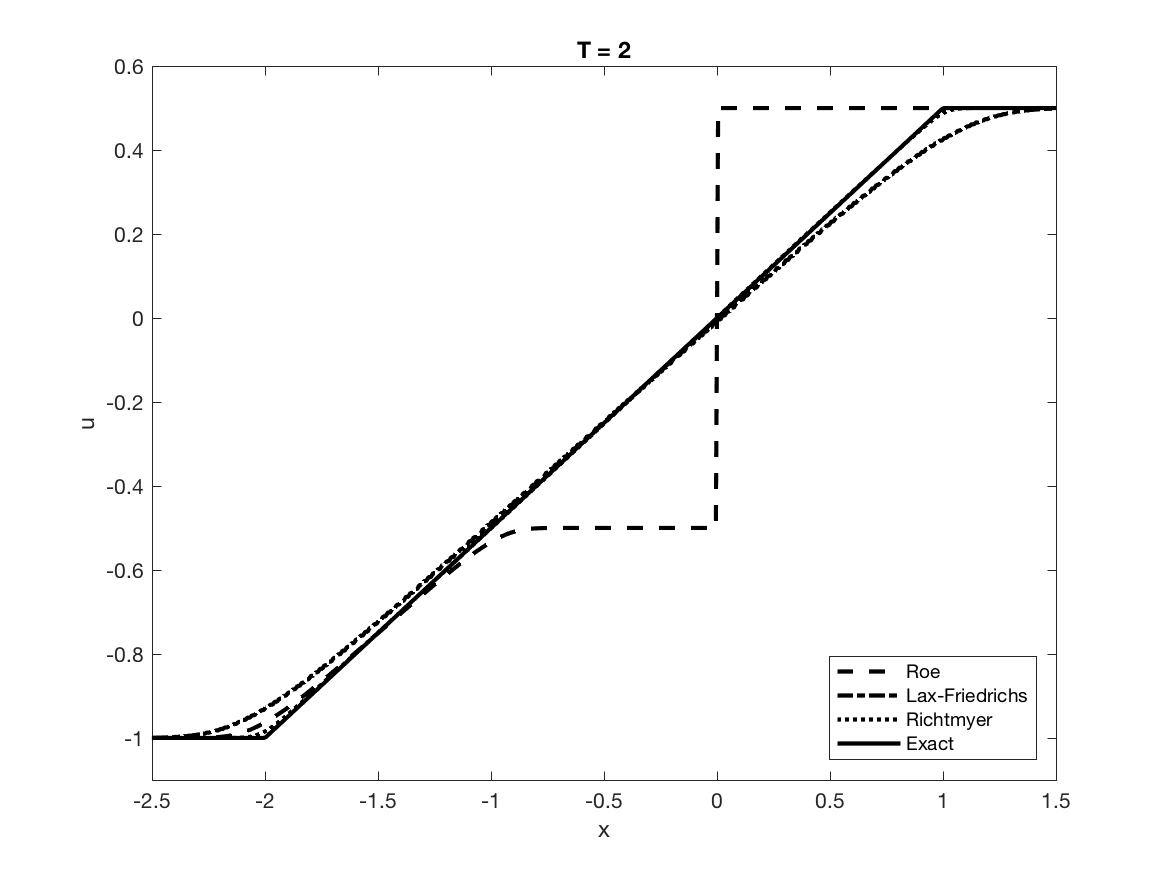
\includegraphics[scale=0.5]{Figures/03_02.png}
      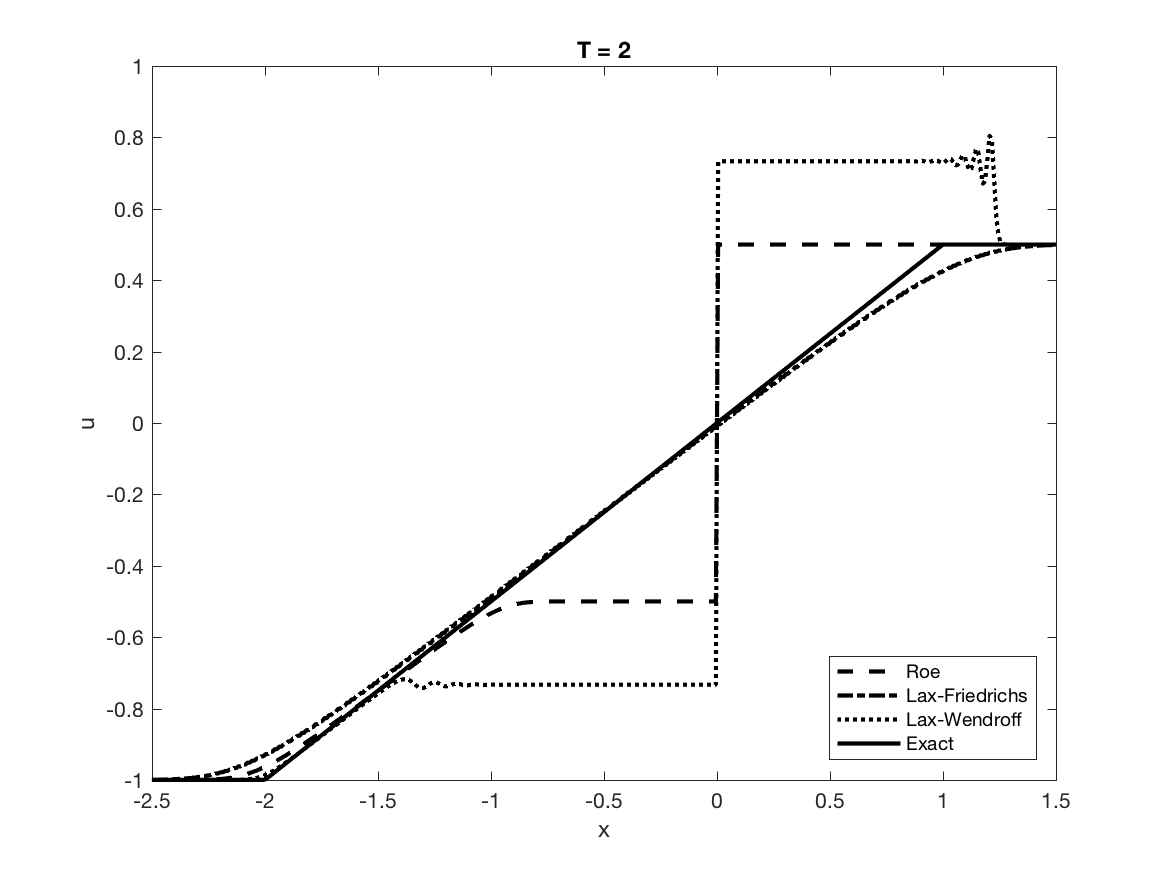
\includegraphics[scale=0.5]{Figures/03_03.png}
    \end{center}

\end{enumerate}
\end{document}
